%追加すべき事項
% - 実験結果の画像の添付
% - DDSP解説
\appendix
\chapter{学習時のパラメータ}
\label{app:params}

提案モデルの学習時のパラメータの値を\prettyref{tab:params1}に示す。また、\prettyref{tab:params2}はAdam~\cite{Adam}で用いるパラメータの値である。

\begin{table}[h]
\centering
\begin{minipage}{0.49\hsize}
    \centering
        \begin{tabular}{lr}\toprule
            パラメータ & 値 \\ \midrule
            バッチサイズ & 1 \\ 
            エポック数 & 1000 \\ \bottomrule
        \end{tabular}
    \caption{}
    \label{tab:params1}
\end{minipage}
\begin{minipage}{0.49\hsize}
    \centering
        \begin{tabular}{lr}\toprule
            パラメータ & 値 \\ \midrule
            $\beta_1$ & 0.5 \\
            $\beta_2$ & 0.999 \\
            $\eta$ & 0.0002 \\ 
            $\epsilon$ & $10^{-8}$ \\ \bottomrule
        \end{tabular}
    \caption{}
    \label{tab:params2}
\end{minipage}
\end{table}

\chapter{データセットの分割}
\label{app:split}

22音ずつの4つのサブセットにデータセットを分割した~(\prettyref{fig:data_div})~。また、データセットの4分割は、88音をシャッフルして配列に格納した後に22音ずつ順に選ぶことで実装した。

\begin{figure}[h]
\centering
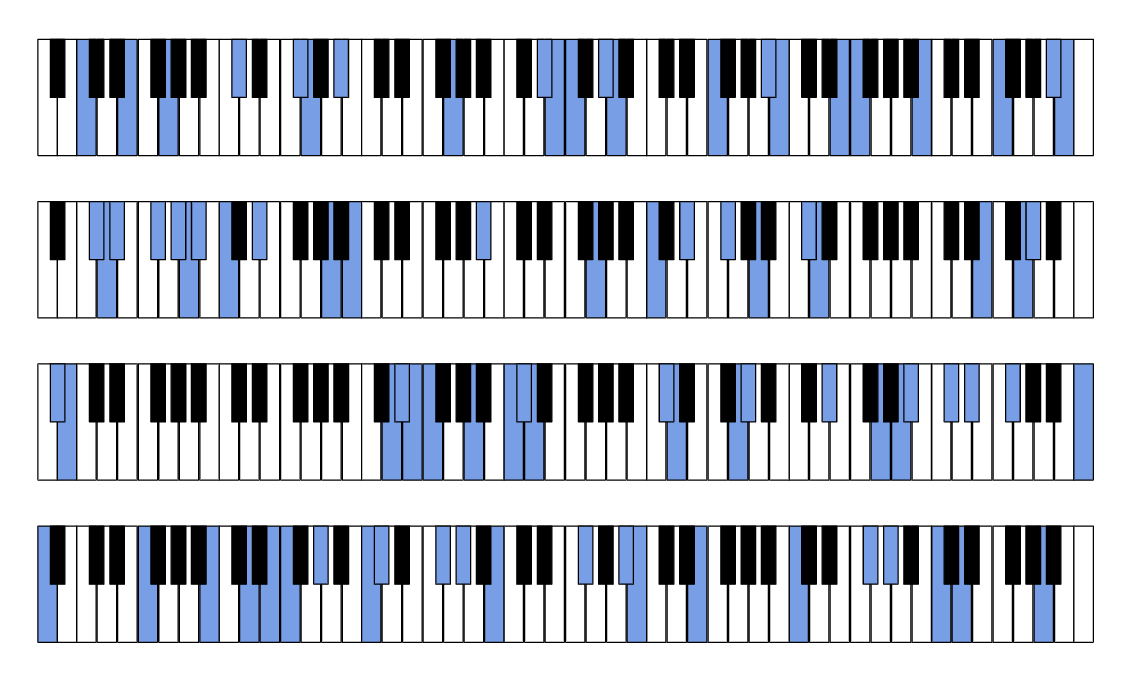
\includegraphics[width=\hsize]{figure/data_div.png}
\caption{データセットのサブセット}
\label{fig:data_div}
\end{figure}

\chapter{DDSP}
\label{app:DDSP}

\chapter{実験結果}
\label{app:result}

\prettyref{sec:result}に載せることのできなかった波形の図を本章に載せる

\section{提案モデルの表現力の評価実験}

提案モデルの評価実験を行ったところ、88音のうち87音については変換先のギターの音を表現できていると判断することができた。


\section{提案モデルの汎化能力の評価実験}